\section{Durchführung}
\label{sec:durchführung}

    Für die Messung der Compton-Wellenlänge $\lambda_\text{c}$ ist die folgende Apparatur gegeben.
    \begin{figure}[H]
        \centering
        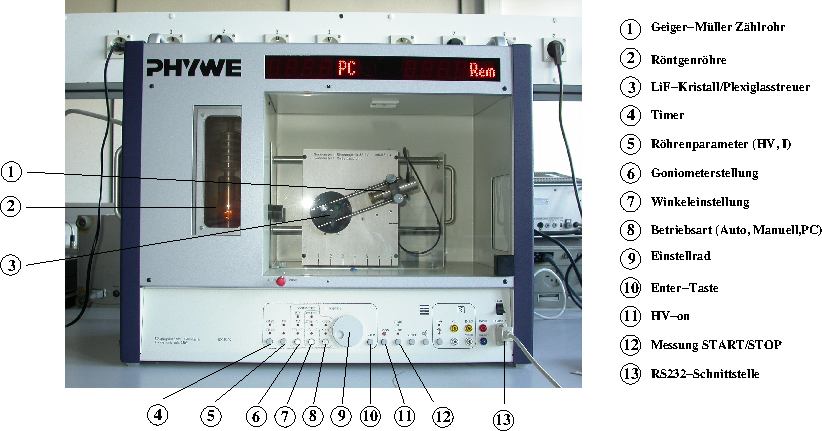
\includegraphics[scale=1]{content/img/Abb_2.pdf}
        \caption{Apparatur zur Erzeugung und Messung von Röntgenstrahlung.}
        \label{fig:aufbau_röntgen}
    \end{figure}
    Innerhalb der Apparatur befinden sich eine Röntgenröhre,
    ein LiF-Kristall, beziehungsweise ein Plexiglasstreuer,
    und ein Geiger-Müller-Zählrohr.\\
    \\
    Die Messung setzt sich aus zwei Teilen zusammen.
    Für alle Messungen wird eine Beschleungungsspannung von $\SI{35}{\kilo\volt}$ eingestellt,
    sowie ein Emissionsstrom von $\SI{1}{\milli\ampere}$.

\subsection{Das Emissionsspektrum der Röntgenröhre}

    Zuerst soll mithilfe des Rechners das Emissionsspektrum der $\ce{Cu}$-Röntgenröhre bestimmt werden.
    Dazu wird das Programm \texttt{measure} ausgewählt,
    in dem unter dem Punkt \texttt{Messgeräte} die Röntgenröhre gesteuert werden kann.\\
    Anschließend wird eine $\SI{2}{\milli\meter}$ Blende und ein LiF-Kristall in die Apparatur eingebaut.
    Nun wird zur Messung des Spektrums der Winkel des LiF-Kristalls in Schritten von $\symup{\Delta}\theta = \SI{0.1}{\degree}$ erhöht mit einer Integrationszeit von $t = \SI{10}{\second}$.

\subsection{Experimentelle Bestimmung der Compton-Wellenlänge}

    Nun soll die Transmission $T(\lambda)$ eines Aluminium-Absorbers untersucht werden.
    Dazu wird der Absorber vor der Blende befestigt.
    In einem Intervall von $\theta = [\SI{7}{\degree}, \SI{10}{\degree}]$ wird in Schritten von $\symup{\Delta}\theta = \SI{0.1}{\degree}$ mit $t = \SI{200}{\second}$ nun die Zählrate gemessen.
    Dabei wird einmal die Zählrate ohne Absorber $N_0(\theta)$ und einmal mit Absorber $N_\text{Al}(\theta)$ gemessen.
    %
    Die Totzeit des Geiger-Müller-Zählrohrs $\tau = \SI{90}{\second}$ erfordert eine Korrektur nach der Gleichung
    \begin{equation*}
        I = \frac{N}{1 - \tau N} \ .
    \end{equation*}
    %Es wurde ja gefragt ob die Korrektur notwendig ist, also müssen wir das ggf streichen
    \\
    Die nächsten Messungen werden ohne das Rechnerprogramm durchgeführt.
    Dazu wird das Röntgengerät auf \texttt{Manuell} umgeschaltet und das RS232-Kabel entfernt.\\
    \\
    Statt des LiF-Kristalls wird nun ein Plexiglasstreuer in die Apparatur eingebaut,
    sowie eine $\SI{5}{\milli\meter}$-Blende.
    Es ist der folgende Aufbau im Inneren der Apparatur aus Abbildung \ref{fig:aufbau_röntgen} gegeben.
    \begin{figure}[H]
        \centering
        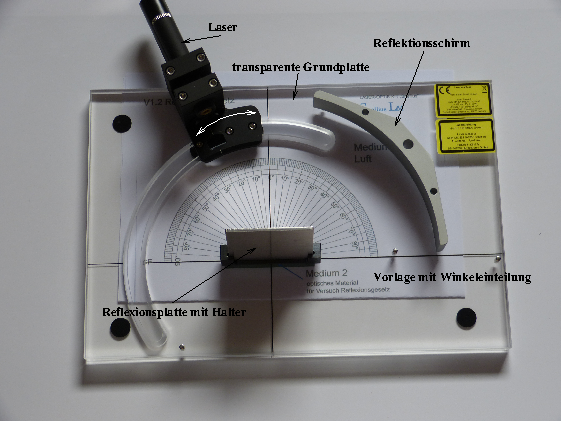
\includegraphics[scale=1]{content/img/Abb_3.pdf}
        \caption{Aufbau zur Messung der Transmission.}
        \label{fig:aufbau_transmission}
    \end{figure}
    Mithilfe der Abbildung \ref{fig:aufbau_transmission} a) wird nun die Transmission $T_1 = \sfrac{I_1}{I_0}$ der ungestreuten Wellenlänge $\lambda_1$ gemessen,
    indem der Plexiglasstreuer in einem Winkel von $\SI{45}{\degree}$ ausgerichtet wird,
    und das Geiger-Müller-Zählrohr in einem Winkel von $\SI{90}{\degree}$ zur Röntgenröhre.
    Nun wird die Intensität $I_0$ ohne den Absorber in einer Zeit von $t = \SI{300}{\second}$ gemessen,
    sowie die Intensität $I_1$ mit dem Absorber,
    welcher zwischen Röntgenröhre und Plexiglasstreuer eingebaut wird.\\
    Für die gestreute Wellenlänge $\lambda_2$ wird die Transmission $T_2 = \sfrac{I_2}{I_0}$ bestimmt.
    Die Intensität $I_2$ wird gemessen, 
    indem der Aluminium-Absorber nach Abbildung \ref{fig:aufbau_transmission} b) zwischen Plexiglasstreuer und Geiger-Müller-Zählrohr angebracht wird.\\
    Aus der Verschiebung der Wellenlänge $\symup{\Delta}\lambda$ kann nun nach den Gleichungen \ref{eqn:wellenlängendifferenz} und \ref{eqn:verschiebung_winkelabhängig} aus Kapitel \ref{sec:compton_effekt} die Compton-Wellenlänge $\lambda_\text{c}$ bestimmt werden.
